
\RequirePackage{fix-cm}

% Document Settings
\documentclass[natbib,twocolumn]{svjour3}


% Flushing
\smartqed


% Packages
\usepackage{graphicx}
\usepackage{xcolor}
\usepackage{amsmath}
\usepackage{multirow}
\usepackage{marvosym}
\usepackage{textcomp}


% Journal Name
\journalname{Journal of Seismology}


% START: The Document
\begin{document}


% Long Title
\title{Seismic Hazard Estimation of Northern Iran Using Smoothed Seismicity}


% Running Title
\titlerunning{Seismic Hazard of Northern Iran}


% Authors
\author{%
	N.~Khoshnevis \and
	S.~Azizzadeh-Roodpish \and
	R.~Taborda \and
	C.~H.~Cramer
}


% Affiliations
\institute{%
	N.~Khoshnevis \and C.~H.~Cramer \at
	Center for Earthquake Research and Information,
	University of Memphis, 3890 Central Ave., Memphis TN 38152, USA\\
	\and
	S.~Azizzadeh-Roodpish \and R.~Taborda (\Letter)\at
	Department of Civil Engineering, and
	Center for Earthquake Research and Information,
	University of Memphis, 3890 Central Ave., Memphis TN 38152, USA\\
	\email{ricardo.taborda@memphis.edu}  
}


% Date
% \date{Received: date / Accepted: date}


% Title Production
\maketitle


% Abstract
\begin{abstract}
	% 
This article presents a seismic hazard assessment for northern Iran where a smoothed seismicity approach has been used in combination with an updated seismic catalog and a recently introduced ground motion prediction equation. We evaluate the hazard over a geographical region including the three major seismic zones affecting the northern part of the country, namely Azerbaijan to the northwest, the Alborz Mountain Range in the northern-central region of Iran, and Kopeh-Dagh to the northeast. For completeness, we also consider the partial contribution of the two remaining seismic zones to the south, that is, Zagros to the southwest, and the south-central and southeastern Iranian seismic zone. Following the concepts of smoothed seismicity, events are not assigned to specific faults but are instead assumed to be potential seismogenic sources by in themselves, and are spatially distributed within regular grid cells of size equal to 0.1\textdegree in both the latitude and longitude directions. After performing the corresponding magnitude conversions, we decluster both historical and instrumental seismicity catalogs to obtain earthquake rates based on the number of events with magnitude greater than 3 within each cell, and smooth the results to account for the uncertainty in the spatial distribution of future earthquakes. Smoothing was done using a Gaussian filter in incremental intervals of magnitude. Seismicity parameters are calculated and smoothed for each region separately, and for comparison purposes, we also consider the combination of all the seismic zones as a uniform region. Seismic hazard curves are first obtained for two distinct models defined on two structural risk scenarios based on the assumption that damage occurs above earthquake magnitude thresholds of $M_w$ greater than 4.5 and 5.0, and then combined into a single one to account for the proportion of reinforced and unreinforced structures. The results are presented in terms of expected peak ground acceleration curves and hazard maps and considering exceedance probabilities of 2 and 10 percent in 50 years for rock site conditions, and compared to equivalent estimations available in the literature at selected locations. Despite some localized differences \textcolor{red}{[???]}, we find our results to be in good agreement with previous results. Therefore, we find the method used here is appropriate to estimate seismic hazard for northern Iran. We conclude with an analysis of the results and its implications for the region, and highlight... or offer some additional thoughts about... \textcolor{red}{[Naeem: what would you say is the main conclusion or major finding?]}.

% Naeem's original abstract

% In this study we conduct a new probabilistic seismic hazard assessment for northern Iran, using recently confirmed ground motion prediction equations and updated seismic catalogs. We evaluate seismic hazard over whole three tectonic seismic zones (Alborz Mountain Range, Azerbaijan and Kopeh-Dagh) and part of two tectonic seismic zones (Zagros and Central-East Iran) using smoothed seismicity. In this model, events are not assigned to specific faults and are assumed to be potential seismogenic sources, spatially gridded to cells. We decluster historical and instrumental seismicity to compute the rate of earthquakes in each grid, and smooth these rates to account for uncertainty in the spatial distribution of future earthquakes. We assume each grid cell has spacing of $0.1^{\circ}$ in latitude and $0.1^{\circ}$ in longitude and count the number of earthquakes in each of them. We use Gaussian filter to smooth the fraction of earthquakes in incremental intervals of magnitude. For this article, in order to consider the seismicity rate, we consider all historical and instrumental earthquakes with magnitude above 3. To calculate the seismic hazard we defined two models based on structural damage threshold magnitude, including Mw 4.5 and Mw 5. Seismicity parameters are calculated for each seismic region, and smoothed seismicity is calculated separately for each. We also consider the combination of regions as a uniform region.  We add the probability of exceedance of all regions and present the smoothed seismicity hazard in northern Iran. The horizontal peak ground acceleration is selected as the ground motion parameter. The results are assessed in terms of the expected peak ground acceleration (PGA) with a 10\% and 2\% probability of exceedance in 50 years for rock site conditions. The seismic hazard map for northern Iran is presented. 
	\keywords{%
		Seismic hazard \and 
		Spatially smoothed seismicity 
		\and Northern Iran
	}
\end{abstract}


% Article Content


\section{Introduction}

This article presents a new seismic hazard assessment for the northern portion of the Iranian plateau, using a smoothed seismicity approach in combination with an updated seismic catalog and a ground motion prediction equation recently evaluated and found to fit well with observations of peak ground response in the region. 

The Iranian plateau is located on the Himalayan-Alpine seismic belt. It is confined between the convergent movements of the Arabian and Eurasian plates, and laterally trapped between the Arabian and eastern Asia-Minor to the west, and the Indian and Eurasian plates to the east \citep{Berberian_1981_Chap}. This entrapment lifts the plateau and gives rise to the three major mountain ranges delimiting Iran's land, the Zagros mountain ranges running from the southeast to the northwest, the Alborz ranges to the north, and the east Iranian ranges. It also defines the seismic activity of the region---one with a long history of large magnitude ($M>7$) earthquakes that are well documented dating back to the \myrevision{eighth} century---which has repeatedly damaged Iran's infrastructure and taken the lives of thousands. \myrevision{(see Fig.~\ref{fig:iran})}

According to this tectonic setting and the geologic provinces of the plateau, Iranian earthquakes have been categorized into various seismic zones, ranging from the definition of four to nine major seismic zones in the more traditional studies \citep[e.g.,][]{Stocklin1968, Takin1972, Berberian1976}, and up to twenty to twenty-three seismotectonic provinces in the most elaborate ones \citep[e.g.,][]{Nowroozi1976, Tavakoli1999}. Contemporary, well-accepted models divide Iran into five major tectonic regions: Azerbaijan-Alborz, Kopeh-Dagh, Zagros, Central-East Iran, and Makran \citep[e.g.,][]{Mirzaei1998}. More recently, in a study aimed to develop a uniform earthquake catalog for Iran, \citet{Karimiparidari2013} further divided the Azerbaijan-Alborz region into two separate seismic zones: Azerbaijan and the Alborz Mountain Range, hereafter referred to simply as Alborz. We adopt the latter definition of six seismic zones and focus our attention on those most relevant to the northern part of the country, Azerbaijan, Alborz and Kopeh-Dagh.

Over the last three decades there have been multiple efforts to better estimate the seismic parameters and hazard, and improve the assessment of seismic risk in Iran \citep[e.g.,][]{Tavakoli1999, Moinfar_2000_Chap, Ghodrati2003, Moinfar_2012_WCEE, Khodaverdian_2016_BSSA}. The most recent of these studies \citep{Khodaverdian_2016_BSSA} focuses \myrevision{on} the estimation of spatially-variable seismic parameters for the whole country using a similar approach to the one we used here. We, however, focus our attention in the northern three seismic zones of the country assuming regionally-based and smoothed seismic parameters. Altogether, these previous studies have helped improve the Iranian Code of Practice for Seismic Resistant Design of Buildings \citep{BHRC2014}. Such improvements are reflected in lower overall expected damage ratios, as reported by \citet{Ghodrati2013} for the city of Tehran. However, other indicators suggest persistent high levels of seismic risk. Therefore, more complete and accurate assessments of seismic hazard---incorporating the latest available data and alternative methods---are still necessary.

Northern Iran houses about 41 percent (32 million) of the total population of the country in the cities of Tehran, Mashhad, Tabriz, Karaj, Qom, Urmia, Rasht, and Ardabil. This region has suffered devastating effects of earthquakes in the past \citep[e.g.,][]{Mehrain_1990_Tech, Chafory-Ashtiany_1999_DPM, Razzaghi_2012_Tech}. Due to its importance, northern Iran has recently been the subject of various efforts to better characterize seismic hazard \citep[e.g.,][]{Abdollahzadeh2014a, Boostan2015}. Among other things, these studies have highlighted the prevailing differences between studies, the importance of quantifying uncertainties, and the need for considering all potential faults in the region---even if believed inactive---by adopting new methodologies and the latest available data.

\myrevision{Most previous studies focus on particular locations  based on specific categorization of seismogenic faults \citep[e.g.][]{Ghodrati2003,Vafai2011,Abdi2013}, which are often subjectively interpreted and limited to data availability.} We use the smoothed seismicity method introduced by \citet{Frankel1995}. This approach has been used with success in other regions \citep[e.g.][]{Cao1996, Akinci2004, Kalkan2009}, including Iran \citep{Khodaverdian_2016_BSSA}. Its major feature is the treatment of cataloged instrumental and historical earthquakes as individual point sources as opposed to events that are part of a predefined system of faults in a given tectonic setting. While we recognize that probabilistic seismic hazard analysis based on fault systems can be more realistic and accurate, by choosing the smoothed seismicity method we seek to \myrevision{acknowledge} the uncertainty associated with fault mapping, earthquake location and source mechanism definitions, and to cover areas that would otherwise be underestimated or ignored. In our analysis, we assume earthquake hazard in northern Iran to be dominated by the seismic zones of Azerbaijan, Alborz, and Kopeh-Dagh, but also consider the contribution of the areas of Zagros and the central-east seismic zones to the hazard calculation within our domain of interest (see Fig.~\ref{fig:iran}). In addition to this five seismic-zone model, we obtain results for the entire region of interest as if it could be considered as a single uniform seismic zone. We used both these models and the combination of them to interpret seismic hazard in northern Iran.

In the following sections we describe our region of interest in greater detail, review its associated tectonics and seismicity, and provide additional information about the adopted approach. Significant aspects of our work include the composition of the earthquake catalog, including catalog completeness and the conversion of earthquake magnitudes, the selection of an appropriate attenuation relationship for the region, and the estimation of the Gutenberg-Richter seismicity parameters. Our analysis includes seismic hazard curves and maps for peak ground acceleration (PGA) considering exceedance probabilities of 2 and 10 percent in 50 years for rock site conditions for events with moment magnitude \myrevision{$M_w \geq 4.5$}. We analyze our results in light of similar estimates available in the literature and summarize the most relevant conclusions.




\begin{figure*}[t] 
	\centering
	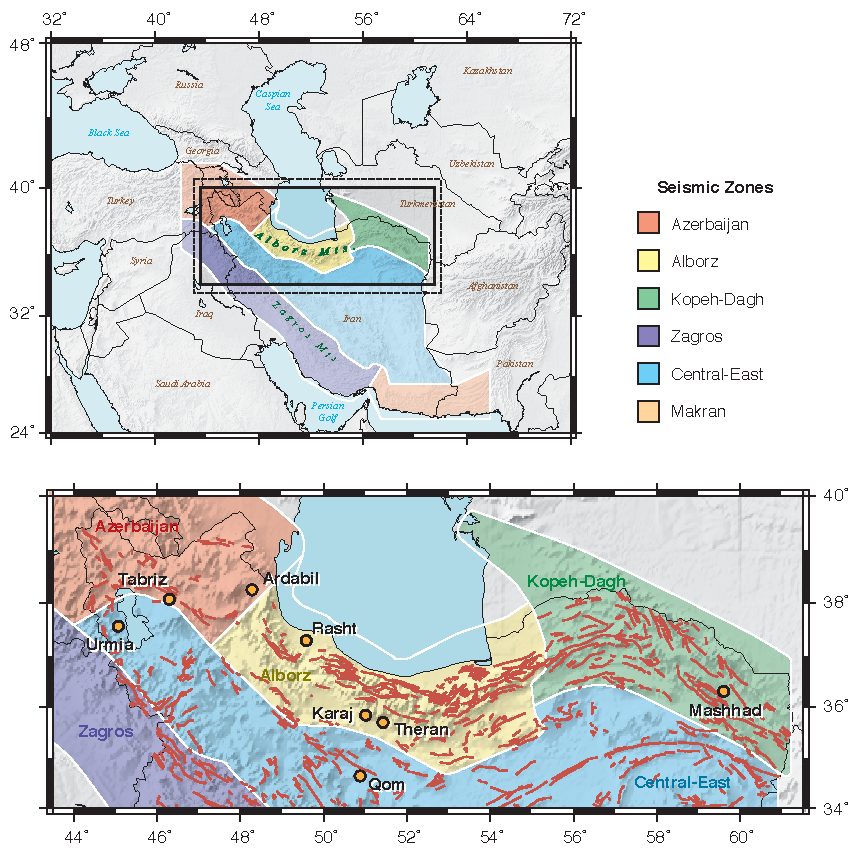
\includegraphics[width=0.9\textwidth]{figures/pdf/figure-01}
	\caption{Region of interest and Iranian seismic zones. At the top, the map of Iran and surrounding countries with shaded relief in the background and the Iranian seismic zones \citep[after][]{Karimiparidari2013} and region of interest in the foreground. The dashed box indicates the complete region of interest and the thicker line box indicates the effective area for which seismic hazard is estimated. The effective region of interest is shown in greater detail at the bottom. Details include the location of the major urban centers and seismic faults in northern Iran.}
	\label{fig:iran}
\end{figure*}

\begin{figure*}[t] 
	\centering
	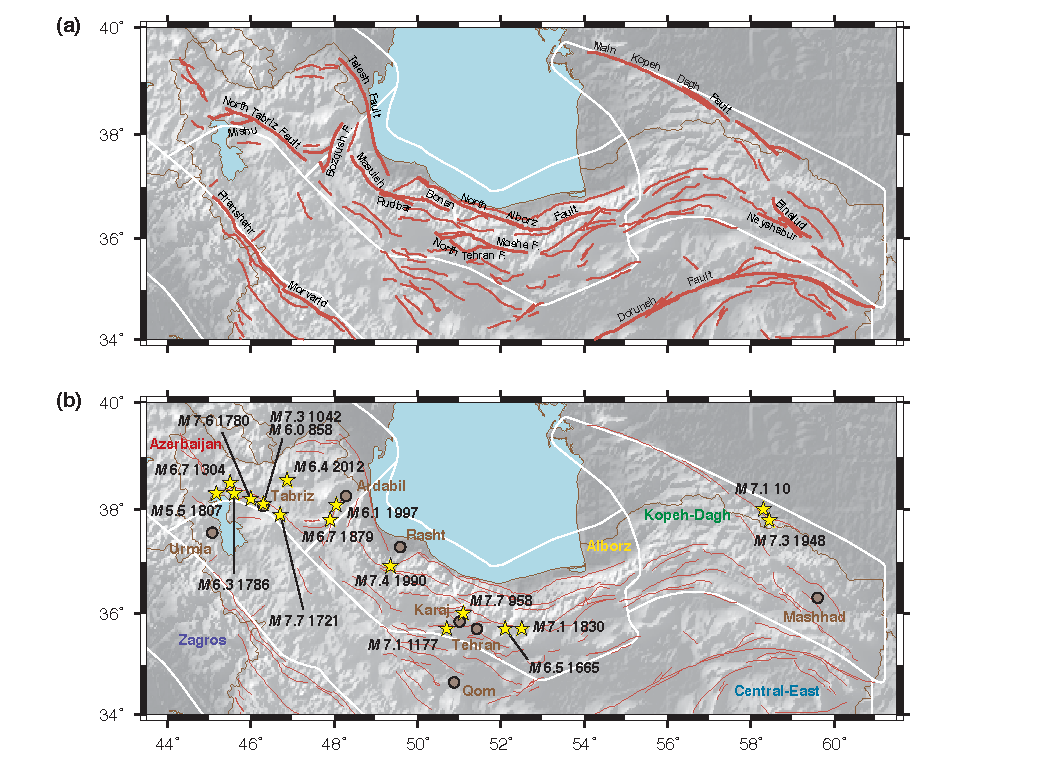
\includegraphics[width=0.9\textwidth]{figures/pdf/figure-02}
	\caption{(a) Main fault line and fault systems, and (b) notable earthquakes in the region of interest. White lines delimit the three major seismic zones in northern Iran. Epicentral locations are indicated with stars. The labels next to each star or linked with a line to avoid congestion show the magnitude and year of the earthquake. The borderlines of the seismic zones shown in Fig.~\ref{fig:iran} are shown in the background in white, along with the light gray shaded relief.}
	\label{fig:selected}
\end{figure*}

\section{Region of Interest}

We define our region of interest between longitudes 43.5\textdegree{}E and 61.5\textdegree{}E, and latitudes 34\textdegree{}N and 40\textdegree{}N, as shown in Fig.~\ref{fig:iran}. These limits correspond to the effective region of interest for which we will present results in subsequent sections. Our calculations, however, included data from a slightly larger region with a \myrevision{2\textdegree{}-perimeter} as indicated in the figure. This is done to avoid the artificial decay effect that results from smoothing the seismicity along and near the edges of the effective region of interest and/or to provide a uniform contribution from the earthquakes surrounding the region \citep[see][]{Lapajne1997}. The effective region has an area of 1,703 km $\times$ 667 km. It encloses the northern part of Iran with most of the Azerbaijan seismic zone, the complete zones of Alborz and Kopeh-Dagh, and the northernmost portions of the Zagros and Central-East seismic zones.

At the \myrevision{northwest} of Iran, the seismic zone of Azerbaijan is strongly controlled by the North Tabriz Fault (NTF) system. This system, shown in Fig.~\ref{fig:selected}a, is a complex northwest-trending structure with a predominant right-lateral, strike-slip faulting mechanism \citep{Berberian1999}. Historical accounts document the occurrence of earthquakes in this area as far back as to the 9th century, with events in the years 858 ($M$ 6.0), 1042 ($M$ 7.3), and 1304 ($M$ 6.7) \citep{Berberian1999}. In the 18th century, in particular, the NTF ruptured three times in a span period of 65 years, which included the $M$ 7.7 1721 Tabriz earthquake in the southeastern section, the $M$ 7.6 1780 Tabriz earthquake in the northwestern section, and the $M$ 6.3 1786 Marand-Mishu on the Mishu reverse fault and the Sufian segment of the NTF. According to \citet{Jones1834}, the \myrevision{1721} Shebli and Tabriz earthquakes had surface ruptures of more than 35 and 42 km, respectively, and the latter presented vertical separations of about 2 to 4 m. The locations of these and other notable events, including the $M$ 5.5 1807 Tasuj and the $M$ 6.7 1879 South Bozqush earthquakes, are shown in Fig.~\ref{fig:selected}b. More recently, the same region was struck by the $M_w$ 6.1 1997 Ardabil and $M_w$ 6.4 2012 Tabriz earthquakes, which caused extensive damage and took the lives of more than 1500 people.

Transitioning from the Azerbaijan to the Alborz seismic zone, the next fault system runs along the Rocks of the Talesh mountains, to the northwest of the Alborz Mountains. Faults in this area have also ruptured recently \citep{Berberian1999}. The $M_w$ 7.4 1990 Manjil-Rudbar earthquake, for instance, caused numerous deaths and significant damage to the region in the south Caspian depression. At the central area of the Alborz seismic zone, near Tehran, the region is characterized by active reverse faults in the North Tehran Thrust (NTT) system (see Fig.~\ref{fig:selected}a for reference). These faults are parallel to the northwest-trending structural gain of the Alborz Mountains belt, and include the south-dipping partially blind faults of Davudieh, Shian, and Bagh-E Feyz. According to \citet{Ambraseys_1982_Book}, Tehran---or the ancient city of Rey---has been devastated in multiple occasions due to severe earthquakes in this area. Historical accounts document the occurrence of multiple $M>7$ earthquakes in 743, 958, 1177, 1665, and 1830. The 1830 earthquake, in particular, ruptured the central segments of the NTT, adjacent to the Mosha fault.

To the east, the Main Kopeh-Dagh Fault is the predominant faulting system in the seismic zone with the same name. This system consists of several partly overlapping segments parallel to a NW--SE oriented structure of step-overs, which exhibits active tectonic displacements along a distance of more than 500 km \citep{Trifonov1978}. The system is also characterized by short south-dipping thrust faults striking E--W \citep{Berberian2001}. The Main Kopeh-Dagh Fault is responsible for the $M_w$ 7.3 1948 earthquake (Fig.~\ref{fig:selected}b). This event struck Ashgabat, the capital city of Turkmenistan, and destroyed more than 30 villages in Iran. Historically, the Kopeh-Dagh seismic zone is also responsible for multiple earthquakes at the boundary between the Neyshabur and Binalud reverse faults (Fig.~\ref{fig:selected}a) between 1209 and 1405 \citep{Berberian1999}, and an estimated $M_s$ 7.1 earthquake in 10 A.D.~\citep{Berberian2001}.

% *********************************************************************************************************************
% *********************************************************************************************************************


% Seismic activity in the Iranian plateau is dominated by the tectonic contacts between the Arabian, Eurasian, and Indian plates, which confine the region laterally between the Indian and Eurasian plates, and the Arabian and eastern Asia-Minor plates to the east and west, respectively. This setting gives rise to the Zagros, Alborz, and east Iranian mountain ranges, and defines the geology of the region. Based on these conditions, Iranian seismicity is typically divided into various seismic zones, varying from as few as four to as many as twenty-three \citep[e.g.,][]{Stocklin1968, Berberian1976, Tavakoli1999}. Here, we adopt the model proposed by \citet{Karimiparidari2013}, which consists of six seismic zones: Azerbaijan, Alborz, Kopeh-Dagh, Zagros, Central-East, and Makram (Fig.~\ref{fig:iran}).

% Within this context, w


% *********************************************************************************************************************
% *********************************************************************************************************************

% Naeem's original Text
% ---------------------

% With respect to different seismicity rates of the regions \citep{Nemati2015}, as well as the completeness of the seismic catalog \citep{Zare2014} , the study region is divided into three tectonic seismic zones. Each of these zones is characterized by its respective seismicity parameters values, including b-value and maximum magnitude ($M{_{max}}$). Part of Central Iran and Zagros regions are inside of the study region. We also calculated the seismicity parameters in these regions. Fig.~\ref{fig:Iran} shows the study region and different seismotectonic classification.

% \begin{figure*}[!ht] 
% \centering
% \includegraphics[scale=0.7]{figures/pdf/Figure1.pdf} 
% \caption{ a) Map of Iran and surrounding countries. The study area is presented in gray box. b) The study area containing seismotectonic provinces after \citet{Mirzaei1998}, and location of big cities. Dashed line is the subdivision that is proposed by \citet{Karimiparidari2013}. }
 
% \label{fig:Iran}
% \end{figure*}

% \subsection{Tectonic Regions and Seismic Faults}

% \subsubsection{Alborz Mountain Range (Alborz)}
% Tehran region has active reverse faults, which are parallel to the northwest-trending structural gain of the Alborz Mountains belt. Here a series of historical earthquakes occurred within a time period of more than 1100 years. Four earthquakes with magnitude more than 7 devastated the Tehran region in four centuries period, from 743 to 1177, but in the last 800 years, only one earthquake at 1830 has struck this region. At least three damaging earthquakes in 958 (western segments), 1655 (eastern segments), and 1830 (central segments), ruptured adjacent segments of the Mosha fault, located in northern Tehran.
% The North Tehran Thrust (NTT) adds more complexity due to the presence of south-dipping reverse faults, which are in part blind, such as the Davudieh, Shian, and Bagh-E Feyz.
% The northwest continuation of the Alborz Mountains, known as the Rocks of the Talesh Mountains, have been thrust northeastward and eastward over rocks of the south Caspian depression. An earthquake with Ms 6.0 in 1978 led to a focal mechanism consistent with a low-angle thrust \citep{Berberian1999}. Recently, the 1990 $M_w$ 7.4 Manjil-Rudbar earthquake caused extensive loss of life and significant damage \citep{USGS_manjil}. Based on existing documents, Tehran city and ancient Rey city have been destroyed completely several times by severe earthquakes with magnitudes greater than 7 \citep{Ambraseys2005}. \\

% \subsubsection{Azerbaijan}
% There were three earthquakes from 1721-86 that ruptured the North Tabriz Fault system from southeast to northwest. The Tabriz region is in the Araxes structural block of northwestern Iran, southwest of the continuation of the western Alborz Mountains towards the Caucasus. The North Tabriz Fault (NTF) is a complex northwest-trending structure, which contains evidence observed on aerial photographs, and vertical displacement with the north side up, of right-lateral strike-slip displacement \citep{Berberian1999}.
% The NTF system and nearby reverse faults ruptured from southeast to northwest in three earthquakes over 65 years: the Shebli earthquake with magnitude 7.3 in 1721 on the southeastern NTF with a surface rupture more than 35 km long, reported by \citet{Jones1834} the Tabriz earthquake with magnitude 7.4 in 1780 on the northwestern NTF, with a surface rupture more than 42 km long and vertical separation of 2 to 4 $m$; and the Marand-Mishu earthquake with magnitude of 6.3 in 1786 on the Mishu reverse fault and the Sufian segment of the NTF. Another earthquake with  magnitude 5.5 struck the Tasuj reverse fault farther west in 1807 and an earthquake of M 6.7 took place along the South Bozqush reverse fault farther southeast in 1879. Prior to the 1721-86 earthquake sequence, Tabriz was shaken by earthquakes in 858 (M 6.0), 1042 (M 7.3), 1273 (M ~ 6.5), and 1304 (M 6.7)\citep{Berberian1999}. Most recently, earthquakes with $M_w$ 6.1 in 1997 and $M_w$ 6.4 in 2012 occurred in Ardabil and Tabriz, respectively. These earthquakes caused around 1500 casualties and extensive damage \citep{USGS_ardabil,USGS_tabriz}.\\


% \subsubsection{Kopeh Dagh}
% The main Kopeh-Dagh fault system has experienced some historic earthquakes. Ashgabat, the capital city of Turkmenistan, was destroyed by an earthquake of Ms 7.2 in 1948 and destroyed more than 30 villages in Iran. This was the strongest earthquake to strike this region since at least 1455.
% The main Kopeh-Dagh fault consists of several partly overlapping segments parallel to the overall $NW - SE$ structure with step-overs. The regions of overlap are characterized by shorter south-dipping thrust faults striking about $E - W$ \citep{Berberian2001}. \citet{Trifonov1978} reported active displacement along the main Kopeh-Dagh fault for more than 500 km. 
% Massive destruction of the capital city of Mithradatkert is attributed to the 10 BC event Ms 7.1, roughly 30 kilometers from the border of Iran (Nesa mound) \citep{Berberian2001}.
% The Neyshabur sequence of four earthquakes between 1209 and 1405 respected the segment boundary between the Neyshabur and Binalud reverse fault system \citep{Berberian1999}.
% Historical records show that in 1209, the district of Neyshabur from Neyshabur city in the west to Daneh village in the east was totally destroyed \citep{Berberian1999}.\\



% \subsection{Historical  and Instrumental Seismicity}
% Uniform earthquake catalog is the most important factor in seismic hazard analysis of a region.  Different studies have been conducted in order to prepare a uniform catalog for Iranian Earthquake. Historical event interpretation and different magnitude conversion relationships are some of the factors which make all these catalogs different. Among different sources \citet{Ambraseys2005}, \citet{Berberian1994}, and \citet{moinfar1994} are some of the main sources for Iranian earthquake catalog. These catalogs contain historical and instrumental earthquakes that have been reported in literature and national and international networks. According to \citet{Ambraseys2005}, there are some scattered indication of earthquake effects  back to third millinuim BC. However, adequate documentary coverage of individual events begins from seventh century A.D. \citet{Mirzaei1997} provided a comprehensive list of studies that have been done in compilation a uniform catalog for Iranian earthquakes in order to prepare a uniform catalog of earthquake (all earthquakes are converted to surface wave magnitude Ms) for seismic hazard assessment in Iran. The catalog is covering the period of 4th century B.C. through 1994. The instrumental data is achievable from three national agencies including IIEES, International Institute of Earthquake Engineering and Seismology; IRSC, The Iranian seismological center, University of Tehran; and BHRC, Building and Housing Research Center (Iran Strong Motion Network) (For more information about these networks see \citet{Karimiparidari2013}).
% Many most of attenuation relationship use  moment magnitude $M_w$ as an input for the equation \citep{Douglas2011}. Moment magnitude is not suffering from saturation and has physical meaning \citep{Kanamori1977}. Due to mentioned reasons Mw has become a most appropriate magnitude scale in recent studies. 
%  \citet{Karimiparidari2013}compiled a uniform earthquake catalog for Iran and adjacent areas, using international and national databanks until April 2010.  They developed relationships between moment magnitude and other magnitude based on orthogonal regression.  They removed the dependent events (aftershocks and foreshocks) using the procedure by \citet{Gardner1974}. The catalog of events with magnitude equal and above Mw 5.5 is provided. 
% \citet{Shahvar2013} presented a unified and homogeneous catalog for the Iranian plateau $(M_w >= 4)$, created by merging data from two local catalogs and seven international agencies for 1900-2011 period. They used orthogonal regression method \citep{Castellaro2006} to derive magnitude conversion relation. By removing foreshocks and aftershocks according to the procedure detailed in Uhrhammer(1986), they also provided declustered version of the catalog.

% The recent unified catalog for Middle East region is published as a part of Global Earth Model (GEM) and the Earthquake Model of the Middle East (EMME) project by \citet{Zare2014}. They used all historical (pre-1900), early and modern instrumental events up to 2006. The catalog contains data from Alborz-Azerbaijan, Afghanistan-Pakistan, Saudi Arabia, Caucasus, Central Iran, Kopeh-Dagh, Makran, Zagros, and part of Turkey. The magnitude of all events are converted to Mw through relationships which is derived at previous studies or newly derived at the study relationships. They declustered data through different methods including \citet{Gardner1974}, Uhrhammer(1986), \citet{Reasenberg1985}, and Gruenthal. \citet{Zare2014} provided the catalog completeness for different magnitude range using  the cumulative frequency-magnitude distribution of  \citet{Gutenberg1944} and \citet{richter1958}, and frequency magnitude distributaion of ZMAP \citep{Wiemer2001} software. The methods confirms the results of each other. 

% In this study we consider earthquakes with Mw equal and greater than 3. Earthquakes with magnitude 3 are not considered as a structural threat, however, the epicenter of earthquakes with magnitude $M_w 3$ are a  susceptible location for future bigger earthquakes.  According to our preliminary data processing based on IIEES data, Iranian catalog for earthquake with magnitude greater and equal 3, is complete from 2005. In order to make sure about the completeness of the catalog, we use IIEES data from 2000. We used the EMME project data provided by \citet{Zare2014} up to 2000. Fig.~\ref{fig:historical} represents the historical data (pre 1900) in the study region. 

% \subsubsection{Magnitude Conversion}

% The catalog of recorded earthquake from 2000-2015 which is downloaded from IIEES is reported the earthquake based on different magnitude scale. We converted the $M_L$, $M_s$, and $mb$ magnitudes through conversion relationships which is defined in \citet{Zare2014}. There also some of data which is recorded in $M_D$ (Duration magnitude). These data are reported by International Seismological Centre (ISC).  \citet{Deniz2010}, developed a set of empirical equations to convert earthquake magnitudes in $mb$, $M_D$, $M_L$ and $M_s$ scales to the $M_w$ scales using orthogonal regression procedure. They used data of earthquake that occurred in Turkey from different data centers including ISC. In this study we use the conversion equation of \citet{Deniz2010} to convert the Md to Mw. Although they defined the equation based on $M_w>=4.5$, we extrapolate the equation for lower magnitude. We believe having those earthquakes, even with small error  in magnitude is important for estimating an accurate "a" value  in Gutenberge-Richter equation.

% \begin{figure*}[!ht] 

% \centering
% 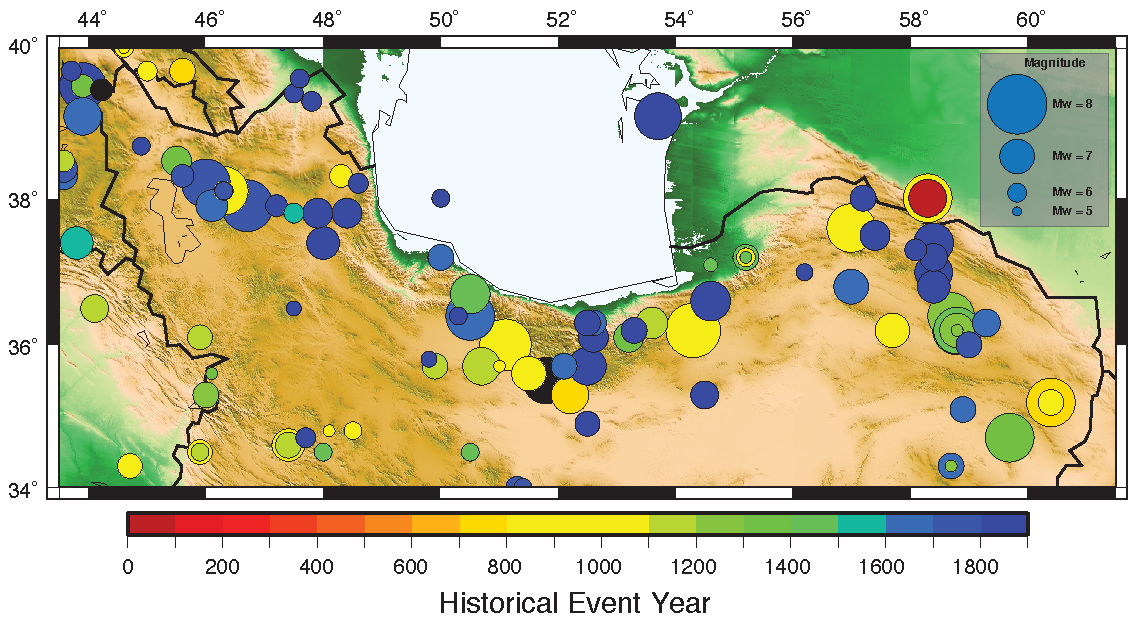
\includegraphics[scale=0.4]{figures/pdf/Figure2.pdf} 
% \caption{Historical earthquakes of Iran (pre 1900). Different colors represent different year of occurrences and size of circles are proportional to the earthquake magnitude. }
% \label{fig:historical}
% \end{figure*}


% \subsubsection{Declustering}

% It is generally assumed that the seismicity of each tectonic seismic source follows a Poissonian occurrence process. Therefore, in order to accomplish this, we declustered the earthquake catalog. In compiling the catalog of events, foreshocks and aftershocks were removed using a declustering methodology \citep{Gardner1974}. For north Iran (lon: 42-62.5, lat: 33-41), from 7478 earthquake event we removed 605 Foreshocks and 2917 aftershocks.
% Whole data that we used for seismicity parameters of Zagros and Central Iran tectonic seismic regions are not included in these numbers. Fig.~\ref{fig:instrumental} shows the epicenter of declustered instrumental  earthquakes.


% \begin{figure*}[!ht] 

% \centering
% \includegraphics[scale=0.25]{figures/pdf/Figure3.pdf} 
% \caption{Declustered instrumental seismicity map (after 1900) of Northern Iran. The study areas are separated at longitude of 48$^{\circ}$ and 55$^{\circ}$ . } 
% \label{fig:instrumental}
% \end{figure*}


% \subsection{Divisions}

% As we discussed earlier (see the Introduction section), classifying the tectonic seismic regions has been a controversial debate. In this study we consider two seismic tectonic models. First model is according to \citet{Mirzaei1998} and \citet{Karimiparidari2013} classification, which includes Azerbaijan, Alborz, Kopek Dagh, and part of Central Iran, and Zagros, the second model is a uniform model for the whole north Iran.  



\section{Seismic Catalog}

\input{compilation}


\subsection{Completeness}

An important aspect of seismic catalogs is their completeness.  Completeness is is measured both in terms of the year of completeness and the completeness magnitude. Both are used in the seismic analysis process. The year of completeness is the point in time at which catalog data exhibits a steady rate of event occurrence. This is measured for different magnitude ranges. A simple approach used by \citet{Frankel1995} and others is to identify the year at which a plot of the cumulative number of events with respect to time becomes (or at least, resembles) a straight line. 

The completeness magnitude, on the other hand, is the minimum magnitude at which the seismic catalog of a region can be considered complete within a certain time period. While the year of completeness can be determined by inspection of the data, the completeness magnitude requires a numerical analysis of the catalog. A common approach is to identify the magnitude associated with the maximum value of the first derivative of the frequency-magnitude curve. This method is widely used as implemented in the ZMAP software package for seismic hazard analysis developed by \citet{Wiemer2001}.

One of the difficulties in determining completeness is the availability of data for a long-enough period of time for all magnitude ranges. In this study, we determined the year of completeness for magnitude ranges 3--4, 4--5, 5--6 and 6--7 by inspection, following the approach used by \citet{Frankel1995}. This is illustrated in Fig.~\ref{fig:completeness}, where we show the cumulative number of events with time for each of the seismic zones and magnitude ranges, and indicate our choice of completeness year thresholds. For events $M_w>7$, in which case there are no sufficient data to determine a proper threshold, we assumed the catalog to be complete from the earliest time at which there is record of large magnitude earthquakes. 

The chosen years of completeness are compiled in Table \ref{tab:completeness}. Also shown in this table are the values of completeness magnitude for each seismic zone and for the uniform model of the entire region of interest. 


... \citet{Zare} provide the years for catalog completeness in their the original catalog for the different regions in their study on the seismicity of the Middle East. They used the 





% For the smoothed seismicity method, completeness of each magnitude in the catalog is an important factor.  \citet{Frankel1995} plotted the cumulative number of events against time for different regions. He assumes that from the point that the line become linear, the catalog is complete. This approach is similar to the MAXC method of ZMAP software \citep{Wiemer2001}, where the completeness treshold is the maximum value of the first derivative of the frequency-magnitude curve. 

% Using the cumulative frequency-magnitude distribution of \citet{Gutenberg1944} and also frequency magnitude distribution approach in software ZMAP, \citet{Zare2014} reported the catalog completeness for the study regions. 

% World widely large earthquakes were routinely located after increasing number of seismic stations establishment in the early 1900s \citep{Shearer2009}. Up to 1961 these data formed the early instrumental period. In 1961 the Worldwide Standardized Seismograph Network (WWSSN) was stablished. The record of these seismographs considerably improved the seismic catalogs in different part of the world \citep{Shearer2009}. Fig.~\ref{fig:completness_scatter} shows the magnitude distribution of events with respect to the time of occurrence of the events.

% We pick the Mw 0.5 increments in magnitude to be able to compare the results with \citet{Zare2014}. In order to be able to compare the results with \citet{Zare2014} we merge the data of Azerbaijan and Alborz seismic regions.  Fig.~\ref{fig:completness_compare_zare_2014_Az_Al} shows the completeness of catalog for earthquakes with different magnitude range in Azerbaijan-Alborz region. According to this figure, midrange magnitudes ($ 4 < Mw < 6 $) fairly obey the network developments in 1900 and 1961. The completeness thresholds for each magnitude range which are reported by \citet{Zare2014} are shown by dashed green line. 

% In this study we follow the \citet{Frankel1995} approach to determine the completeness of each region. Even though the approach used by \citet{Frankel1995} will lead to the conservative results, we make sure that we don't use a period of time without knowing the complete number of events. Determining the completeness of the catalog is very sensitive to the data. Converting earthquake magnitudes from different scales to moment magnitude obviously has some error. Having broader range of magnitude will help to minimize these sort of error. In this study we consider the magnitude intervals for completeness study as $Mw = 1$. 


\begin{figure*}[t]
    \centering
    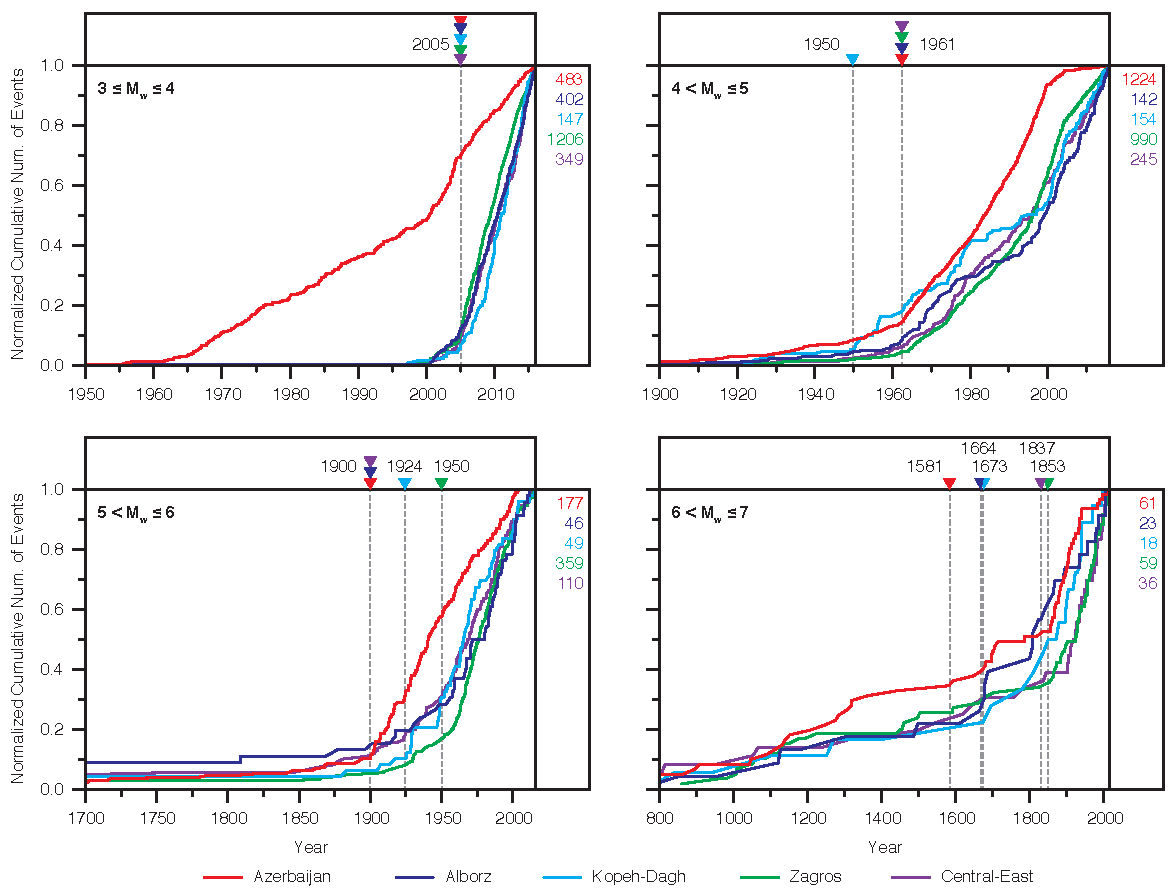
\includegraphics[scale=0.28]{figures/pdf/figure-05.pdf} 
    \caption{Pending.}
    \label{fig:completeness}
\end{figure*}

\begin{table}[t]
    \centering
    \caption{Year thresholds and magnitude completeness for the seismic zones within the region of interest in this study.}
    \begin{tabular}{@{\hspace{0.2ex}}lccccrc@{\hspace{0.2ex}}}
        \cline{2-7}                                              \\[-1.6ex]
                        & 3--4 & 4--5 & 5--6 & 6--7 & 
                                  \multicolumn{1}{c}{$>7$} &$M_c$\\[0.6ex]
        \hline                                                   \\[-1.6ex]
        Azerbaijan      & 1961 & 1961 & 1900 & 1581 & 1042 & 4.5 \\
        Alborz          & 2005 & 1950 & 1900 & 1664 &--401 & 4.4 \\
        Kopeh Dagh      & 2005 & 1950 & 1900 & 1673 &    9 & 4.5 \\
        Zagros          & 2005 & 1961 & 1900 & 1853 & 1439 & 4.4 \\
        Central-East    & 2005 & 1961 & 1854 & 1837 &  762 & 4.5 \\
        Uniform Model   & 2005 & 1961 & 1900 & 1778 &--401 & 4.5 \\[0.5ex]
        \hline 
    \end{tabular}
    \label{tab:completeness} 
\end{table}





\section{Seismic Hazard Approach}

There have been multiple assessments of seismic hazard for Iran. A brief report on the most recent review done to define the hazard zoning map of Iran included in the Iranian seismic code \citep{BHRC2014} can be found in \citet{Moinfar_2012_WCEE}. Other previous efforts include, for instance, the work of \citet{Tavakoli1999}, who presented iso-acceleration contour lines and seismic hazard zonation for Iran based on known major fault-lines and area-source models; the results obtained by \citet{Ghodrati2003}, who presented a refined hazard assessment for the metropolitan area of Tehran using a logic tree approach to combine results from three attenuation relationships; and the recent study by \citet{Khodaverdian_2016_BSSA}, who used a smoothed seismicity approach to estimate spatially variable seismicity parameters for the whole country.

Once a seismic catalog has been defined, the second most important step is precisely the definition of the seismicity parameters $a$ and $b$ used in the Gutenberg-Richter recurrence relation 
% 
\begin{equation}
	\log_{10} N = a - b M \, ,
\end{equation}
% 
\noindent
where $N$ is the number of earthquakes with magnitude greater than or equal to $M$, $a$ accounts for the number of earthquakes that occur within a given region, and $b$ is a measure of the occurrence of earthquakes relative to magnitude \citep{Gutenberg1944}. These parameters can be assumed constant or variable depending on the approach used. 

In this study we use the smoothed seismicity method introduced by \citet{Frankel1995}. This method has been used successfully in different regions around the world including Alaska, California, Hawaii, Italy, Turkey \citep[e.g.,][]{Cao1996, Klein2001, Akinci2004, Kalkan2009, Moschetti2014}. In it, the $b$-value is commonly assumed constant within a given seismic zone of ``homogeneous'' seismogenic characteristics, whereas $a$ is varied spatially according to the cataloged occurrence of earthquakes. The spatial variation of $a$ is defined based on dividing the region of interest into regular-size grid cells. The parameter $a$ is determined based on the number of events $n_i$ within each cell $i$ of magnitude greater than a reference value $M_{\mathrm{ref}}$, and discretized in different magnitude ranges (or bins). The number of earthquakes within each cell is then smoothed spatially taking into account the values of neighboring cells using a Gaussian function. In essence, the smoothed seismicity approach addresses the aleatoric uncertainty of future earthquake locations by using a weighted contribution of the background regional seismicity, and thus eliminates the need for knowledge about specific fault locations.

In this study we discretize the region of interest into a regular grid with cells of size 0.1\textdegree{} $\times$ 0.1\textdegree{} (in longitude and latitude). The parameter $a$ for each cell is obtained based on the information in the seismic catalog described in the previous section. Following \citet{Frankel1995}, $n_i$ is smoothed using the normalized Gaussian function
% 
\begin{equation}
	\tilde{n}_i = \frac
		{ \sum_{j} n_{j} \exp ( \frac{ -\Delta_{ij}^{2} }{ c^2 } ) }
		{ \sum_{j} \exp ( \frac{ -\Delta_{ij}^{2} }{ c^2 } ) }
	\, ,
	\label{eq:nnorm}
\end{equation}
% 
where $\tilde{n}_i$ is the smoothed, normalized number of events in cell $i$, $\Delta_{ij}$ is the distance between the $i$-th and $j$-th cells, and $c$ is the correlation distance. The summations in Eq.~\ref{eq:nnorm} are calculated over the number of $j$ cells within a distance $3c$ from the $i$-th cell. It should be noted that in this process we convert the cumulative number of events to incremental values following \citet{Herrmann1977}. We also note that according to \citet{Frankel1995}, moderate earthquakes generally occur in areas where there have been significant numbers of events with magnitudes $M \geq 3$, thus our interest in having complemented the earthquake catalog for events above this threshold.

It is obvious from Eq.~\ref{eq:nnorm} that an important parameter in smoothing the seismicity is the correlation distance. Different values of $c$ have been used in past studies, ranging between 10 and 50 km. \citet{Frankel1995} and \citet{Boyd2008} assumed a correlation distance of 50~km, \citet{Foteva2006} used 10 and 15 km, \citet{Barani2007} used 25~km, and \citet{Khodaverdian_2016_BSSA} used 40 km. According to \citet{Mirzaei1997}, determining an appropriate value of $c$ depends on the crustal structure of the region, the distribution of stations, and the number and quality of records. We use an intermediate value of $c=30$~km. This selection is consistent with epicentral uncertainty for previous hazard zoning maps for Iran \citep[see][]{Zare2012}.

In turn, we consider the $b$-values to be constant within each seismic zone as delimited in Fig.~\ref{fig:iran}. Details about the calculation of the $b$-value for each zone are provided below. By contrast, in the recent work by \citet{Khodaverdian_2016_BSSA}, the authors computed spatially-variable $b$-values within large grid-cells of size 1\textdegree{} $\times$ 1\textdegree{} based on the average seismicity within a 200-km radius from each cell. While gridding $b$-values and considering the influence of neighboring large-size cells allows to draw information from the background seismicity, it is unavoidable to have the contributing areas cross over seismic zones of different characteristics, which may pollute the computation of $b$-values. Admittedly, these are subjective decisions and any reasonable choice can be considered valid or within the margins of the associated epistemic uncertainty.

Last, the annual rate $\lambda$ of exceeding a reference ground motion $u_o$ is defined by
% 
\begin{align}
	\lambda & \left( u > u_o \right) = \nonumber \\
		& \sum_{k} \sum_{l} 10^{ {}^{ \left[ \log \left( \frac{ N_{k} }{ T } \right) - b \left( M_l - M_{\mathrm{ref}} \right) \right] } }
		P \left( u > u_o | D_k , M_l \right)
		\, .
	\label{eq:exceed}
\end{align}
% 
Here, the values of $\tilde{n}_i$ have been previously binned by their distance from the site of interest, $N_k$ is the total of $\tilde{n}_i$ values for cells within a certain bin distance, $T$ is the time in years used to determine $N_k$, and $k$ and $l$ are the indexes of the distance and magnitude bins, respectively. $P ( u > u_o | D_k , M_l )$ is the probability of $u$ exceeding $u_o$ given an earthquake of magnitude $M_l$ at a distance $D_k$ \citep{Frankel1995}.

It is clear from Eq.~\ref{eq:exceed} that the hazard calculations depend also on the choice of an attenuation relationship to obtain predict the level of ground motion at a site ($u$) for any given earthquake. In the following two sections we describe how we obtained the $b$-values for the different seismic zones influencing the hazard in northern Iran and our choice of a suitable attenuation relationship (ground motion prediction equation).


% *********************************************************************************************************************
% PENDING TO USE
% *********************************************************************************************************************

% We are attempting to assess the relative likelihood of moderate earthquakes ($M_w > 4.5$), which cause structural damage. 

% Since the catalog's completeness for $M_w > 3$ and $M_w > 4$ are different, we use two magnitude completeness range for less than $M_w 5$. 

% Earthquake greater than magnitude 5, most probably will occur near where they have occurred in the past.

% According to Building and Housing Research Center \citep{BHRC2014}, $M_w 5$ is considered as a threshold magnitude for onsetting the structural damage. 

% In the smoothed seismicity method, the model uses each event location as a point source, hence $M_w 4.5$ could be damaging earthquake for old masonry buildings or even engineering building if it is very close to it, 

% in this study, in order to consider the probabilistic seismic hazard, we defined two models based on $M_w 5$ and $M_w 4.5$ as a threshold magnitude for seismic hazard calculation.

% *********************************************************************************************************************
% ALREADY USED
% *********************************************************************************************************************

% Occurrence of devastating historical earthquake and also essential needs for constructing new buildings and infrastructures inspired researchers to study the seismic hazard of northern Iran from different points of view. Dividing Iran into 20 tectonic seismic regions, \citet{Tavakoli1999} prepared iso-acceleration contour lines and seismic hazard zonation for return periods of 75 and 475 years corresponding to 50\% and 10\% probability of exceedance in 50 years, based on major known lines and area source models. According to their study, North Tabriz fault zone and north of Tehran fault zone have the highest acceleration. Maximum mean acceleration in the vicinity of these tectonic elements is predicted to be around 0.45 $g$ and 0.3 $g$ for a return period of 475 and 75 years, respectively. In the smaller scale, using the logic tree approach to compensate for uncertainties in the attenuation relationship, \citet{Ghodrati2003} presented a probabilistic seismic hazard assessment of metropolitan Tehran, the capital of Iran. The results showed that the PGA ranges from 0.27-0.46 $g$ for a return period of 475 years and from 0.33-0.55 $g$ for a return period of 950 years. 
% In this study we use background seismicity to estimate the seismic hazard in northern Iran. Using background seismicity, \citet{Cao1996} conducted a seismic hazard estimation study in southern California. They concluded that one could obtain similar results implementing background seismicity to those obtained by introducing zones for areas with well-recorded seismicity patterns. \citet{Lapajne1997} used spatially smoothed seismicity modeling to acquire a seismic hazard outlook in Slovenia. They defined 4 different models with different correlation distances, including a model based of the total released seismic energy. They gained an acceptable PGA in comparison with other seismic hazard approaches. \citet{Akinci2004} estimate the seismic hazard in central and northern Italy using smoothed historical seismicity. Their results showed that the smoothed seismicity approach gives reasonable regionalized results without introducing seismogenic zones. This approach has also been used in many regions with different seismicity patterns \citep{Wesson1999, Klein2001, Hamdache2003, Kalkan2009, Moschetti2014, Boyd2008}.

% \subsection{Analysis Method}

% \subsubsection{smoothed seismicity method}

% We use spatially smoothed seismic hazard analysis \citep{Frankel1995} to estimate the seismic hazard. 
% In this model, seismic events are spatially gridded to cells. 
% We are attempting to assess the relative likelihood of moderate earthquakes ($M_w > 4.5$), which cause structural damage. 
% % According to \citet{Frankel1995}, moderate earthquakes generally occur in areas that there have been significant numbers of events of magnitude 3 and above. 
% % Therefore, these events provide a reasonable guide to where moderate earthquakes will most likely occur. 
% Since the catalog's completeness for $M_w > 3$ and $M_w > 4$ are different, we use two magnitude completeness range for less than $M_w 5$. 
% Earthquake greater than magnitude 5, most probably will occur near where they have occurred in the past.
% According to Building and Housing Research Center \citep{BHRC2014}, $M_w 5$ is considered as a threshold magnitude for onsetting the structural damage. 
% In the smoothed seismicity method, the model uses each event location as a point source, 
% hence $M_w 4.5$ could be damaging earthquake for old masonry buildings or even engineering building if it is very close to it, 
% in this study, in order to consider the probabilistic seismic hazard, we defined two models based on $M_w 5$ and $M_w 4.5$ as a threshold magnitude for seismic hazard calculation.
% In order to calculate the annual rate ($\lambda$) of exceeding ground motion ($u$) at a specific site, according to \citet{Frankel1995}, first we need to divide the region into cells (0.1*0.1) and count all earthquake events which are bigger than $M_{ref}$ in each cell. 
% We use Herrmann formula \citep{Herrmann1977} to convert the cumulative (i.e. number of events bigger than $M_{ref}$) values to incremental (i.e. number of events from$M_{ref}$ to $M_{ref}+\Delta_m$) values. 

% Using Gaussian function we smooth the number of events in each cell. The smoothed value $\tilde{n}_i$ is obtained from

% \begin{equation}
% \tilde{n_i}=\frac{\sum_{j} n_{j} e^{\frac{-\Delta_{ij}^{2}}{c^2}}}{\sum_{j} e^{\frac{-\Delta_{ij}^{2}}{c^2}}},
% \end{equation}

% \noindent
% where,  $\tilde{n}_i$  is normalized to preserve the total number of events. $\Delta{_i{_j}}$ is the distance between the $i{_t{_h}}$ and $j{_t{_h}}$ cell. The sum is calculated over cells $j$ within a distance of $3c$ of cell $i$.

% Then we discretized the magnitude and distance in uniform bins and get the total number of Normalized, smoothed events ($N_k$) inside the certain distance increment.

% Having ($N_k$) and $T$ (catalog time duration that we calculated $N_k$ within that duration), we can calculate the annual rate  $\lambda (u> u_0 )$ of exceeding ground motion according to 

% \begin{equation}
% \begin{split}
% \lambda(u>u_{0}) = \sum_{k}\sum_{l}10^{[log(\frac{N_{k}}{T}-b(M_l-M{_r{_e{_f}}}))]} \\
% p(u>u_0 | D_k ,M_l),
% \end{split}
% \end{equation}

% \noindent
% where $k$ and $l$ are denoted as index of distance and magnitude bin. $P(u>u_0 | D_k,M_l )$ is the probability that for an earthquake at distance $D_k$ with magnitude $M_l$, u at the site will exceed  ground motion $u_0$. This probability depends on the attenuation relation and the standard deviation (aleatory variability) of the ground motion for any specific distance and magnitude \citep{Frankel1995}.


% *********************************************************************************************************************
% OLD STUFF
% *********************************************************************************************************************

%%% My (Naeem) original text


%\subsection{Background}
%
%Regarding historical earthquakes and the need for constructing new buildings and infrastructure, different seismic hazard analyses were conducted in Iran. Dividing Iran into 20 tectonic seismic regions, \citet{Tavakoli1999} prepared iso-acceleration contour lines and seismic hazard zonation for return periods of 75 and 475 years or 50\% and 10\% probability of exceedance in 50 years, based on major known lines and area source models. According to their study, North Tabriz fault zone and north of Tehran fault zone are in the highest acceleration contour. Maximum mean acceleration in the vicinity of these tectonic elements is predicted to be around 0.45 $g$ and 0.3 $g$ for a return period of 475 and 75 years, respectively. In the smaller scale, using the logic tree approach to compensate for uncertainties in the attenuation relationship, \citet{Ghodrati2003} presented a probabilistic seismic hazard assessment of metropolitan Tehran, the capital of Iran. The results showed that the PGA ranges from 0.27-0.46 $g$ for a return period of 475 years and from 0.33-0.55 $g$ for a return period of 950 years. 
%In this study we use background seismicity to calculate the seismic hazard.Using background seismicity, \citet{Cao1996} conducted a seismic hazard estimation study in southern California. They concluded that one could obtain similar results implementing background seismicity to those obtained by introducing zones for areas with well-recorded seismicity patterns. \citet{Lapajne1997} used spatially smoothed seismicity modeling to acquire a seismic hazard outlook in Slovenia. They defined 4 different models with different correlation distances, including a model based of the total released seismic energy. They gained an acceptable PGA in comparison with other seismic hazard approaches. \citet{Akinci2004} estimate the seismic hazard in central and northern Italy using smoothed historical seismicity. Their results showed that the smoothed seismicity approach gives reasonable regionalized results without introducing seismogenic zones. This approach has also been used in many regions with different seismicity patterns \citep{Wesson1999, Klein2001, Hamdache2008, Kalkan2009, Moschetti2014, Boyd2008}.
%
%\subsection{Analysis Method}
%\subsubsection{smoothed seismicity method}
%To calculate the seismic hazard, we use spatially smoothed seismic hazard analysis \citep{Frankel1995}. In this model, seismic events are spatially gridded to cells. We are attempting to assess the relative likelihood of moderate earthquakes ($M_w > 4.5$), which cause structural damage. According to \citet{Frankel1995}, moderate earthquakes generally occur in areas that there have been significant numbers of events of magnitude 3 and above. Therefore, these events provide a reasonable guide to where moderate earthquakes will most likely occur. Since the catalog's completeness for $M3+$ and $M4+$ is different, we use two magnitude completeness range for less than $M_ w5$ . Category 5+ and others ($M6+$ and $M7+$) assume that future $M_w 4.5$ events will occur near where they have occurred in the past. \\
%\noindent
%According to Building and Housing Research Center  \citep{BHRC2014}, $M_w5$ is considered as a threshold magnitude to structural damage. In the smoothed seismicity method, the model uses each event location as a point source, hence $M_w4.5$ could be damaging earthquake for old masonry buildings or even engineering building if it is very close to it, in this study, in order to consider the probabilistic seismic hazard of both models, we defined two models based on $M_w 5$ and $M_w 4.5$ as a threshold magnitude for seismic hazard calculation. \\
%\noindent
%\noindent
%In order to calculate the annual rate ($\lambda$) of exceeding ground motion ($u$) at a specific site, according to \citet{Frankel1995}, first we need to divide the region into cells (0.1*0.1) and count all earthquake events which are bigger than $M_{ref}$ in each cell. We use Herrmann formula \citep{Herrmann1977} to convert the cumulative (i.e. number of events bigger than $M_{ref}$) values to incremental (i.e. number of events from$M_{ref}$ to $M_{ref}+\Delta_m$) values. Using Gaussian function we smooth the number of events in each cell. The smoothed value $\tilde{n}_i$ is obtained from
%
%\begin{equation}
%\tilde{n_i}=\frac{\sum_{j} n_{j} e^{\frac{-\Delta_{ij}^{2}}{c^2}}}{\sum_{j} e^{\frac{-\Delta_{ij}^{2}}{c^2}}},
%\end{equation}
%
%\noindent
%where,  $\tilde{n}_i$  is normalized to preserve the total number of events. $\Delta{_i{_j}}$ is the distance between the $i{_t{_h}}$ and $j{_t{_h}}$ cell. The sum is calculated over cells $j$ within a distance of $3c$ of cell $i$.\\
%\noindent
%Then we discretized the magnitude and distance in uniform bins and get the total number of Normalized, smoothed events ($N_k$) inside the certain distance increment.
%Having ($N_k$) and $T$ (catalog time duration that we calculated $N_k$ within that duration), we can calculate the annual rate  $\lambda (u> u_0 )$ of exceeding ground motion according to 
%
%\begin{equation}
%\begin{split}
%\lambda(u>u_{0}) = \sum_{k}\sum_{l}10^{[log(\frac{N_{k}}{T}-b(M_l-M{_r{_e{_f}}}))]} \\
%p(u>u_0 | D_k ,M_l),
%\end{split}
%\end{equation}

%\noindent
%where $k$ and $l$ are denoted as index of distance and magnitude bin. $P(u>u_0 | D_k,M_l )$ is the probability that for an earthquake at distance $D_k$ with magnitude $M_l$, u at the site will exceed  ground motion $u_0$. This probability depends on the attenuation relation and the standard deviation (aleatory variability) of the ground motion for any specific distance and magnitude \citep{Frankel1995}




\begin{figure*}[t]
    \centering
    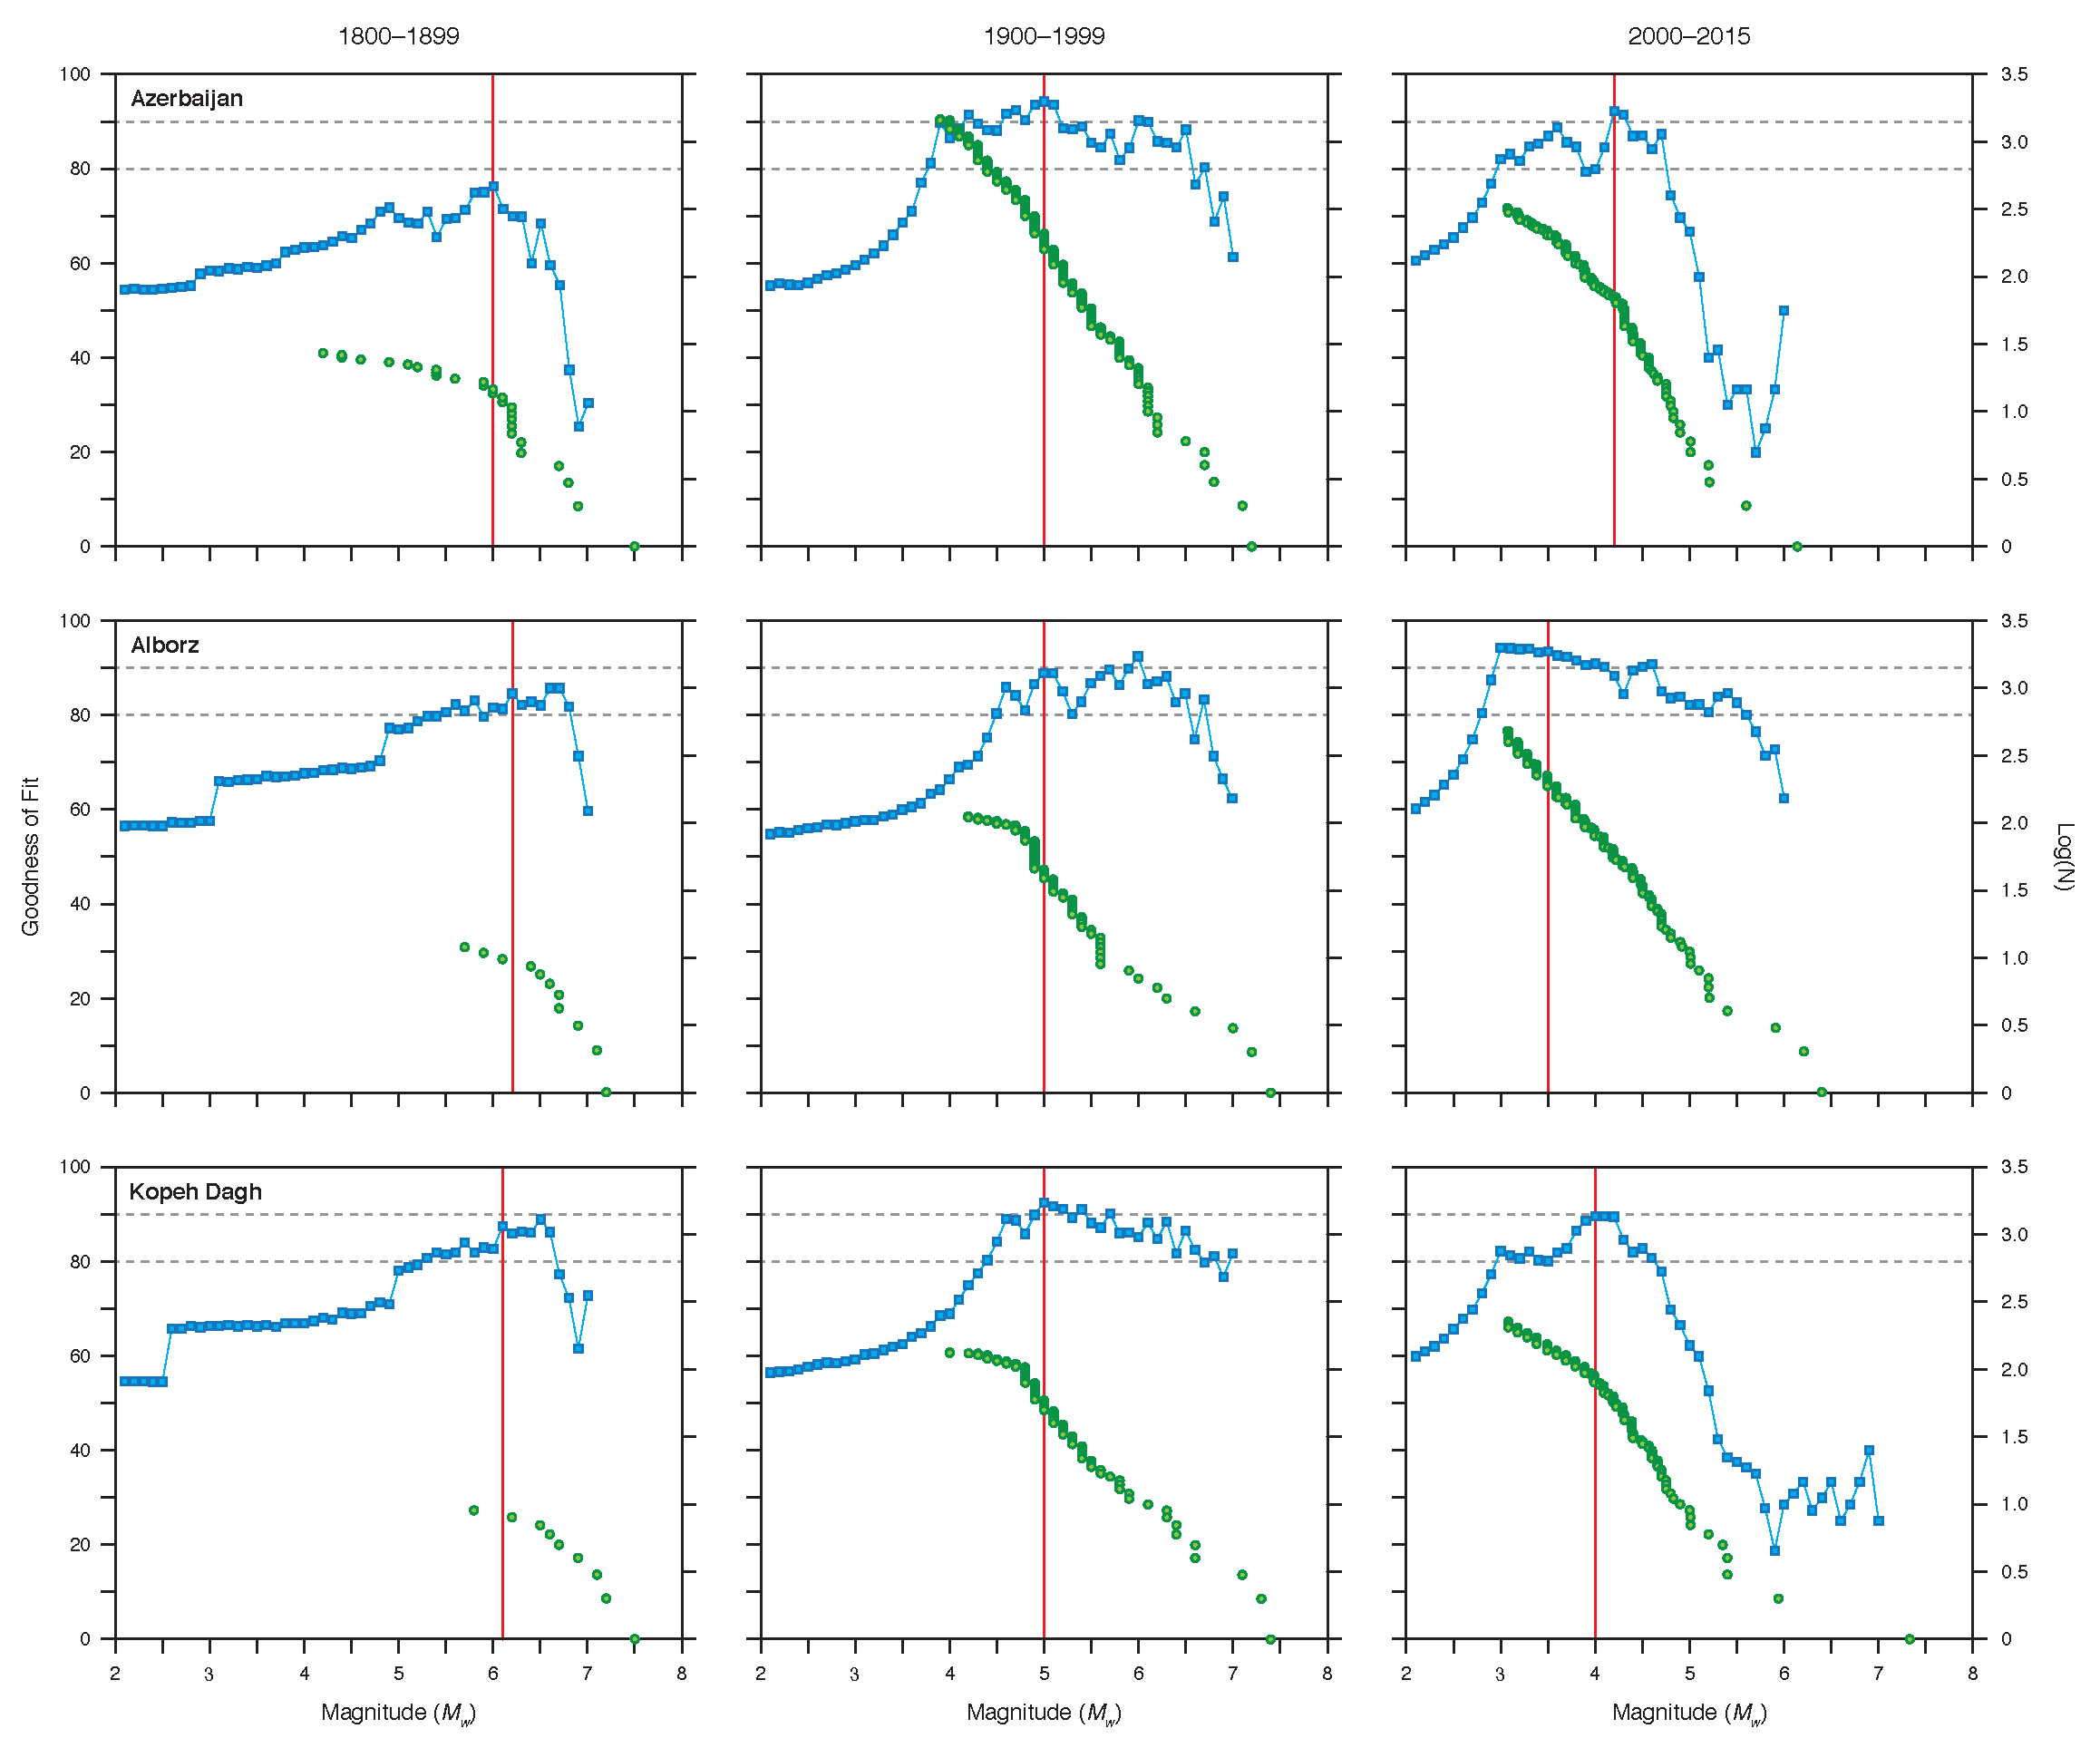
\includegraphics[width=\textwidth]{figures/pdf/figure-06} 
    \caption{Annual probability of exceedance as a function of earthquake magnitude for the seismic zones in the region of interest. The three curves in red correspond to those seismic zones completely considered within the study area, whereas the ones in blue are the two additional contributing zones from the rest of the country. THe last curve in green corresponds to the complete region of interest, here referred to as the uniform model. The shaded range indicates the models' $\pm 1$ standard deviation.}
    \label{fig:annualp}
\end{figure*}

\section{Seismicity Parameters}

Following the general approach described in the previous sections and using the information collected about the seismic catalog and its completeness, we computed the seismicity parameters $a$ and $b$, and the maximum magnitude $M_{\max}$ using the seismic hazard assessment software HA3 (version 3). This software implements the procedures developed by \citet{Kijko_1989_BSSA, Kijko_1992_BSSA}, and subsequent updates by \citet{Kijko_2004_PAG}. HA3 is widely used for this type of computations and is regarded as a reliable tool in seismic hazard analysis \citep[see, for instance,][]{}\textcolor{red}{[references needed]}.

The $a$-value is estimated based on the completeness year, the correlation distance, and the (smoothed) number of events per grid cell. We count events with magnitude $M_w > 3$ and smooth the number of events for each cell. This means each cell has a different $a$-value and thus the result is variable throughout our region of interest. On the other hand, we consider the $b$-value and $M_{\max}$ to be constant within each of the seismic zones in our study area. We compute $b$ and $M_{\max}$ for two different models using the information from the catalog for prehistorical, historical, and instrumental seismicity and the computed values of $M_c$. In the first model we obtain these parameters independently for each one of the five seismic zones influencing the hazard in northern Iran. That is, we obtain distinct values of $b$ and $M_{\max}$ for the main northern seismic zones of Azerbaijan, Alborz, and Kopeh Dagh, as well as for the portions of the Zagros and Central-East seismic zones contributing to our region of interest (see Fig.~\ref{fig:iran} for reference). 

In the second model we consider the whole study area as a uniform seismic zone. Admittedly, this assumption is unrealistic if considered from the point of view that different seismic zones have different seismicity parameters. Nonetheless, computing results for this uniform model is useful for the analysis of results and comparisons with other studies. Table \ref{tab:params} shows the parameters $b$ and $M_{\max}$ obtained with HA3 for the five seismic zones and the uniform regional model, along with the observed maximum magnitude, $M_{\max}^{\mathrm{obs}}$; and Fig.~\ref{fig:annualp} shows the annual probability of exceedance as a function of earthquake magnitude.

\begin{table}[t]
    \centering
    \caption{Seismicity parameters $b$ and $M_{\max}$ computed for the seismic zones in our region of interest and the reference uniform seismicity model along with the observed maximum magnitude, $M_{\max}^{\mathrm{obs}}$.}
    \begin{tabular}{@{\hspace{0.2ex}}lccc@{\hspace{0.2ex}}}
        \cline{2-4}                                                                         \\[-1.6ex]
                        & $b$-value         & $M_{\max}$        & $M_{\max}^{\mathrm{obs}}$ \\[0.6ex]
        \hline                                                                              \\[-1.6ex]
        Azerbaijan      & 1.10 $\pm$ 0.03   & 7.93 $\pm$ 0.34   & 7.7                       \\
        Alborz          & 1.03 $\pm$ 0.03   & 7.85 $\pm$ 0.66   & 7.8                       \\
        Kopeh Dagh      & 0.89 $\pm$ 0.04   & 7.78 $\pm$ 0.31   & 7.6                       \\
        Zagros          & 0.99 $\pm$ 0.02   & 7.47 $\pm$ 0.26   & 7.4                       \\
        Central-East    & 0.95 $\pm$ 0.04   & 7.84 $\pm$ 0.34   & 7.6                       \\
        Uniform Model   & 0.90 $\pm$ 0.02   & 7.87 $\pm$ 0.26   & 7.8                       \\[0.5ex]
        \hline 
    \end{tabular}
    \label{tab:params} 
\end{table}

% *********************************************************************************************************************
% OLD
% *********************************************************************************************************************

% For each of the three seismic regions, Gutenberg-Richter parameters and maximum magnitude ($M_{max}$) were calculated using Seismic Hazard Assessment code (HA3) \citep{kijko2004}. The regional maximum magnitude for each region is estimated by the \citet{Kijko1989} method, which is implemented in the HA3 package. For smoothed seismicity areas, $b-value$ is assumed constant. The $a-value$ can vary spatially and is determined by counting earthquakes above $M$ 3.0 in each grid cells.

% \citet{Karimiparidari2013} applied the Maximum Curvature (MAXC) technique \citep{Wyss1999, Wiemer2000} by ZMap \citep{Wiemer2001} to calculate the level of completeness of instrumental part of the catalog.  Following the \citet{Karimiparidari2013}, we assume the catalog is complete for earthquakes with magnitude 4.5, 4.4, 4.5, 4.5, and 4.4 for Azerbaijan, Alborz,  Kopeh-Dagh, Central Iran, and Zagros tectonic seismic regions, respectively. For the uniform model we used 4.5 as a completeness magnitude. In this study we use those magnitudes of completeness as the magnitude threshold in the calculation of the seismicity parameters. We also used the seismicity parameters of \citet{Karimiparidari2013} as the priory information in HA3 code. The updated values are displayed in Table \ref{tab:b_value}.  Annual occurrence rate of the earthquake for each region is shown in Fig.~\ref{fig:annual_m}.

% *********************************************************************************************************************
% OLDER
% *********************************************************************************************************************

% For each of the three seismic regions, Gutenberg-Richter parameters and Max magnitude ($M_{max}$) were calculated using Seismic Hazard Assessment code (HA3) \citep{kijko2004}. The regional maximum magnitude for each region is estimated by the \citet{Kijko1989} method, which is implemented in the HA3 package. For smoothed seismicity areas, $b-value$ is assumed constant. The $a-value$ can vary spatially and is determined by counting earthquakes above $M$ 3.0 in grid cells.\\

% \citet{Karimiparidari2013} applied the Maximum Curvature (MAXC) technique \citep{Wyss1999, Wiemer2000} by ZMap \citep{Wiemer2001} to calculate the level of completeness of instrumental part of the catalog. In this study we use those magnitudes of completeness as the magnitude threshold in the calculation of the seismicity parameters. We also used the seismicity parameters of this study \citep{Karimiparidari2013} as the priory information in HA3 code. The updated values are displayed in Table 2.

% Following the \citet{Karimiparidari2013}, we assume the catalog is complete for earthquakes with magnitude 4.5, 4.4, and 4.5 for Azerbaijan, Alborz and Kopeh-Dagh tectonic seismic regions, respectively. The completeness of each region can be seen easily from the scatter plot of completeness test. 


\begin{figure*}[t]
    \centering
    \includegraphics[width=\textwidth]{figures/pdf/attenuation.pdf} 
    \caption{Variation of horizontal peak ground acceleration (PGA) with distance. KG2004: \citet{Kalkan2004}, BA2008: \citet{Boore2008}, AB2010: \citet{Akkar2010}, SO2012: \citet{Soghrat2012}. The dashed line are $\pm$uncertainty of KG2004.}
    \label{fig:att}
\end{figure*}

\begin{figure*}[t]
    \centering
    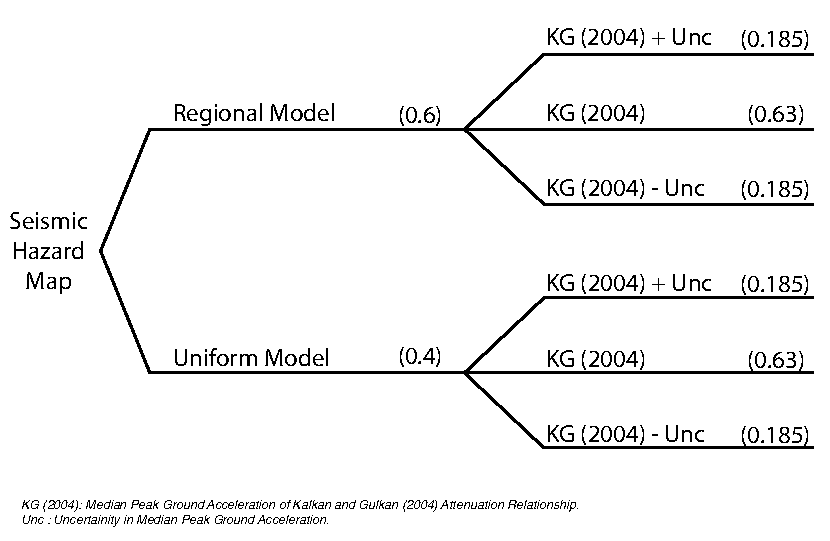
\includegraphics[width=\textwidth]{figures/pdf/logic.pdf} 
    \caption{Logic tree for seismic hazard component in the North Iran.}
    \label{fig:logic}
\end{figure*}



\section{Attenuation Relationship}

The last piece in our hazard analysis process is the choice of an adequate attenuation relationship, or ground motion prediction equation (GMPE). This is a highly influential factor because it controls \myrevision{the intensity level at a particular site given earthquake locations and magnitude from the source model.}

Recently, \citet{Zafarani2014} investigated the predictive capabilities of a set of nine local, regional, and next generation attenuation (NGA) GMPEs to determine their applicability for northern Iran. They evaluated GMPE predictions against data from 32 earthquakes of magnitudes $M_w$ ranging between 4.7 and 7.4. This included comparisons of PGA and response spectral accelerations (SA) computed from time-series recorded on 163 stations located at epicentral distances of up to 200 km. The evaluation was done using the likelihood (LH) and log-likelihood (LLH) methods of \citet{Scherbaum_2004_BSSA, Scherbaum_2009_BSSA}. The combined evaluation for PGA, and SA for seven periods (T) between 0.1 and 2.0 s, yielded that the best overall predictions were those of the GMPEs introduced by \citet{Ghasemi_2009_JS}, \citet{Abrahamson_2008_ES}, and \citet{Chiou2008}. For the specific case of PGA ($T=0$ s), however, the best results were those obtained with the GMPEs introduced by \citet{Kalkan2004}, \citet{Chiou2008}, and \citet{Boore2008}. \myrevision{\citet{Soghrat2012} and \citet{Akkar2010} are other attenuation relationships which provide higher scores.}

Since our hazard analysis here focuses on PGA values only, we concentrated our attention in the last set of GMPEs. In comparisons not shown here for brevity, we found that these GMPEs yielded mean predictions that were very close to each other.\myrevision{ Fig.~\ref{fig:att} illustrates the variation of horizontal components pga (in g) with distance for four different magnitude. In practice, epistemic uncertainty is being considered by using different GMPEs through logic tree approach. As \citet{Atkinson2014} suggested, in most cases multiple-GMPEs approach is not necessarily acknowledge the epistemic uncertainty. This fact is also obvious from the Fig.~\ref{fig:att} where the alternative approach which is using \citet{Kalkan2004} as a backbone GMPE as well as uncertainties covers a broader range in compare with using the combination of GMPEs.} Furthermore, based on the LLH coefficients reported by \citet{Zafarani2014}, and using the \myrevision{approach} of \citet{Scherbaum_2009_BSSA}, we found that a logic-tree analysis \myrevision{led} to weights of 0.3376, 0.3354, and 0.3270 for \citet{Kalkan2004}, \citet{Chiou2008}, and \citet{Boore2008}, respectively. These results meant that neither of them had a substantial advantage over the others. \myrevision{Fig.~\ref{fig:logic} represents the total logic tree approach in order to consider the uncertainty in tectonic seismic region, $M_{max}$, $b-value$, and estimated PGA. The weights are chosen based on previous studies \citep[e.g.,][]{Petersen2015}. We considered the uncertainty in tectonic seismic region through adding the uniform model with lower weight than the most recent accepted classification.}

Based on this, we selected the GMPE proposed by \citet{Kalkan2004} for our analysis. This equation is of the form
% 
\begin{align}
	\ln \left( Y \right) =
		& \hspace{1ex} b_1 + b_2(M_w - 6) + b_3 \left( M_w - 6 \right)^{2} \nonumber \\ 
		& + b_5 \ln \left( r \right) + b_V \ln \left( V_S / V_A \right)
	\, ,
\end{align}
% 
where $Y$ is a ground motion parameter (here representing PGA), $V_A$ is a reference velocity in m/s, \myrevision{and} $V_S$ is the shear wave velocity of the site of interest. In this equation, the distance $r$ is given by
% 
\begin{equation}
	r= \sqrt{ r^2_{\mathit{cl}} + h^2 }
	\, ,
\end{equation}
% 
where $r_{\mathit{cl}}$ is the horizontal distance to the site of interest and $h$ is a reference fictitious depth, both given in km. According to \citet{Kalkan2004}, in the case of $Y$ representing PGA, the coefficients $b_1$, $b_2$, $b_3$, $b_5$ and $b_V$ are
% 
\begin{equation}
\begin{array}{lcrlcr} 
	b_1 &=&  0.393   \,,&\hspace{2em}   b_2 &=& 0.576\,,   \\
	b_3 &=& -0.107   \,,&\hspace{2em}   b_5 &=& -0.899\,,  \\
	b_V &=& -0.200   \,; 
	\nonumber
\end{array}
\end{equation}
% 
and $V_A$, $V_S$ and $h$ are
% 
\begin{equation}
\begin{array}{lcrl} 
	V_A &=& 1,112 & \mathrm{m/s}	\\
	V_S &=&   700 & \mathrm{m/s}	\\
	h   &=&  6.91 & \mathrm{km}\,,
	\nonumber
\end{array}
\end{equation}
% 
respectively. The standard deviation of the residuals $(\sigma_{\ln y})$ expressing the random variability of the ground motions is 0.612. The value of $V_S$ is assumed to represent average surface rock sites.

We should note here that even though \citet{Kalkan2004} derived the above attenuation relationship for distances $r$ up to 250 km, \citet{Zafarani2014} only used data up to 200 km in their evaluation of the various GMPEs available. Therefore, to be consistent with the latter, we set the models in the hazard analysis to compute ground motions (i.e., PGAs) at distances no greater than 200 km.




\begin{figure*}[t]
    \centering
    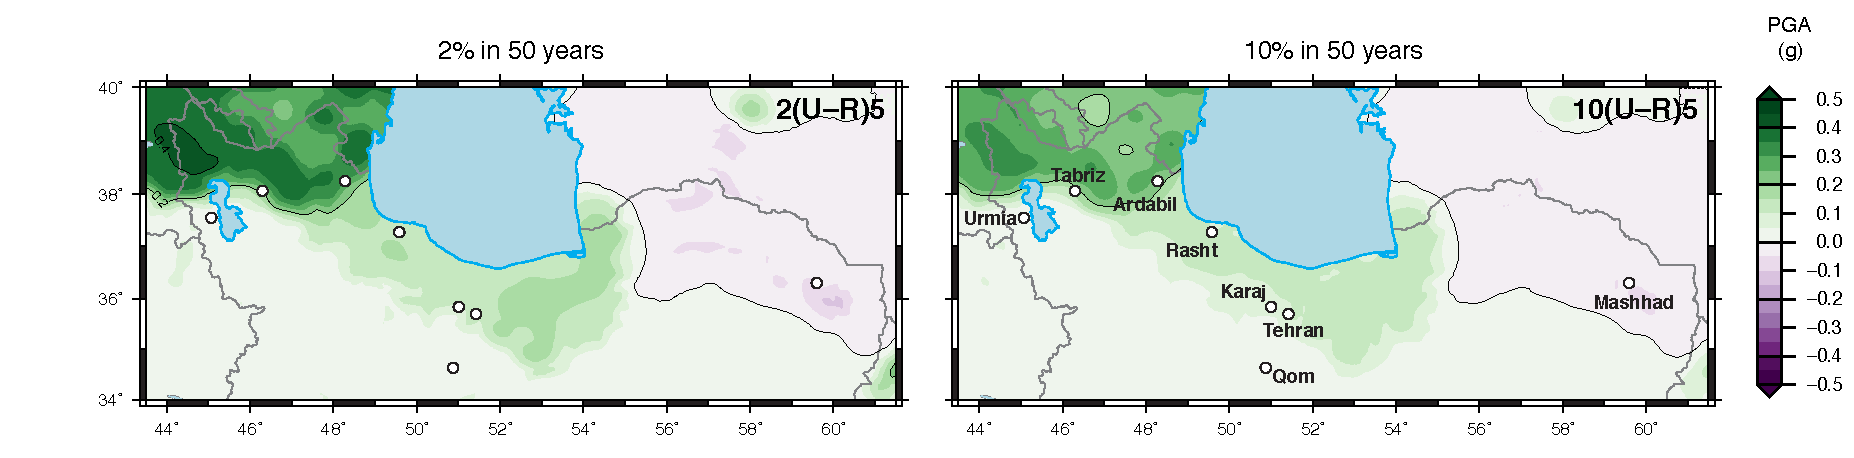
\includegraphics[width=\textwidth]{figures/pdf/figure-09}
    \caption{Logic tree nodes and associated weights used in the seismic hazard analysis for northern Iran.}
    \label{fig:logic}
\end{figure*}

\section{\myrevision{Logic Tree}}

\myrevision{As mentioned in previous sections, we address the uncertainties in our models, seismic parameters and selected ground motion prediction equation via a logic tree. Fig.~\ref{fig:logic} shows the complete set of branches at each of the tree nodes. In particular, we consider uncertainty in the seismic zonation via the combination of the R and U models, the maximum magnitude $M_{\max}$, the seismic $b$-value, and the prediction of PGA intensities in the GMPE by \citet{Kalkan2004}. We assigned the weights to the R and U model arbitrarily, giving more weight to the regional model R based on the expectation that a regionalized model would likely lead to a better seismic hazard analysis. Other weights in the logic tree are based on previous studies \citep[e.g.,][]{Petersen2015}.}

\myrevision{Among other possible parameters for which we could have consider additional sources of uncertainty, we note that we did not consider the variability of the reference depth and seismic velocities in the selected GMPE because these were values fixed to satisfy the fit of the equation with data from northern Iran. Thus introducing uncertainty in these parameters would have been to the detriment of the prediction of PGA values.}

 % We considered the uncertainty in tectonic seismic region through adding the uniform model with lower weight than the most recent accepted classification.}



\section{Results}

The PGA hazard maps have been computed for a 10\% and 2\% exceedance probability in 50 years, corresponding to a return period of 475 and 2475 years, from gridded values of historical and instrumental seismic activity. These levels of exceedance are a standard practice in seismic designs \citep{BHRC2014}.


\section{Conclusions}

The result of a new probabilistic seismic hazard assessment for northern Iran using updated seismic catalogs is provided. Seismic hazard is evaluated over entire three regions (Azerbaijan, Alboz, Kopeh-Dagh) as well as part of Central and Zagros tectonic seismic regions using the smoothed background seismicity. In order to determine the seismic hazard in North Iran, different studies have been done. These studies are based on defining faults as a seismic source model. Using faults as a seismic source model could result in accurate values in case the faults are precisely determined. There are considerable uncertainties on fault characteristic, specially on fault length. Instead of using faults as a seismic source, we consider each earthquake event as a point source in the model. We reduce the uncertainty in earthquake location by smoothing the number of earthquake in adjacent cells. We defined models based on considering the whole North Iran as a uniform seismic tectonic regions and 5 different seismic tectonic regions. The differences in catalog completeness, b value, and maximum magnitude of earthquake in these two models resulted in different results. This indicate the idea that dividing regions into subregions is necessary in order to be able to get accurate results. The result are also sensitive to the minimum magnitude. The structures built according to engineering code are supposed to withstand the earthquake with magnitude 5 at the reasonable distance. However, closer $M_w > 4.5$ for those structures and also older masonry structures could cause structural damage. A combination of two models $(M_w > 4.5, M_w>5)$ in each city based on number of engineering and old masonry structures will provide more accurate results. The results are provided for mean peak horizontal acceleration in bedrock. The ground acceleration in soil deposits and inside basin will be bigger than the provided values. This model reduce the epistemic uncertainty regarding the recognizing faults and earthquake location. Combination of this model with a study based on using faults will increase the values for existing non-active seismic fault regions.  


\section{Acknowledgements}

The authors wish to express their gratitude to Art Frankel at the U.S.~Geological Survey (USGS) for providing access to the Smoothed Probabilistic Seismic Hazard Analysis software and to Morgan Moschetti, also at the USGS, for providing advise on the use of the software. The authors also thank Andrzej Kijko at the University of Pretoria for providing access to the software for computing the seismicity parameters; and Mehdi Zare at the International Institute of Earthquake Engineering and Seismology (IIEES) in Tehran for kindly providing the original catalog data and for his assistance in interpreting previous catalog information. Access to data provided by IIEES is also greatly appreciated. This research was possible thanks to support by the Center for Earthquake Research and Information (CERI) at the University of Memphis. CERI is designated as a Center of Excellence by the Tennessee Board of Regents and is funded in part by the State of Tennessee under State Sunsent Laws (SB 1510 and HB 1608, 2015--2016).
 



% Bibliography
\bibliographystyle{spbasic}
\bibliography{references}
% \nocite{*}


% END: The Document
\end{document}

